\documentclass[11pt]{article}
\usepackage{udec-pset}
\guia{3}{Ley de Gauss}
\mostrarSoluciones
\begin{document}
\crearEncabezado

\section*{Contenidos}

\begin{boxTeoria}{Ley de Gauss (Definición Integral)}
    Establece que el flujo neto de un campo vectorial de tipo ``fuente'' a través de cualquier superficie cerrada es proporcional a la magnitud de las fuentes contenidas en su interior.

    En su forma más general, la ley relaciona el vector densidad de flujo eléctrico $\vec{D}$ con la carga libre total:

    \begin{equation*}
        \Psi_E = \oint_{S} \vec{D} \cdot d\vec{A} = Q_{f, enc}
    \end{equation*}

    A partir de este principio, se desprenden los siguientes puntos fundamentales:
    \begin{itemize}
        \item \textbf{Carga como fuente:} La existencia de un flujo neto distinto de cero implica necesariamente la presencia de fuentes (cargas positivas) o sumideros (cargas negativas) dentro de la superficie.
        \item \textbf{Independencia de la geometría:} El flujo total depende exclusivamente del valor de la carga encerrada, no de la forma de la superficie $S$ ni de la posición de la carga en su interior.
        \item \textbf{Materiales Lineales:} En materiales isotrópicos y homogéneos, la densidad de flujo se relaciona directamente con el campo mediante la relación constitutiva $\vec{D} = \epsilon \vec{E}$, donde $\epsilon$ representa la permitividad propia de cada región.
    \end{itemize}
\end{boxTeoria}

\begin{problema}[Campo Eléctrico debido a una Esfera]
    Considere una esfera de radio $R_2$ compuesta por dos materiales dieléctricos con carga distribuida uniformemente: \\[5pt]

    \begin{minipage}{0.3\textwidth}
        \begin{itemize}
            \item \textbf{Región I} ($0 < r < R_1$): \\ Permitividad $\epsilon_1$, densidad $\rho_1$.
            \item \textbf{Región II} ($R_1 < r < R_2$): \\ Permitividad $\epsilon_2$, densidad $\rho_2$.
            \item \textbf{Región III} ($r > R_2$): \\ Vacío ($\epsilon_0$).
        \end{itemize}
    \end{minipage}
    \hfill
    \begin{minipage}{0.6\textwidth}
        \centering
        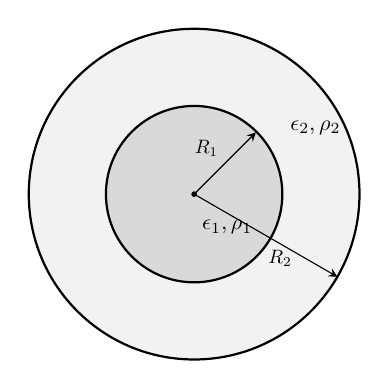
\begin{tikzpicture}[scale=1.4]
            \draw[fill=gray!10, thick] (0,0) circle (1.5);
            \draw[fill=gray!30, thick] (0,0) circle (0.8);
            \draw[fill=black] (0,0) circle (0.02);

            % Usamos "stealth-" y "-stealth" en lugar de flechas con ">"
            \draw[-stealth] (0,0) -- (0.56, 0.56) node[midway, above left, scale=0.7] {$R_1$};
            \draw[-stealth] (0,0) -- (1.3, -0.75) node[pos=0.6, below, scale=0.7] {$R_2$};

            \node[scale=0.8] at (0.3, -0.3) {$\epsilon_1, \rho_1$};
            \node[scale=0.8] at (1.1, 0.6) {$\epsilon_2, \rho_2$};
        \end{tikzpicture}
    \end{minipage}
\end{problema}

\begin{solucion}
    Mediante el uso de la Ley de Gauss, analizaremos cada caso por separado.

        {\bfseries \large Caso 1: $0<r<R_1$.}
    Inicialmente, se debe escoger una superficie donde aplicar la Ley de Gauss, la superficie escogida para problemas esféricos corresponde, valga la redundancia a una esfera, la esfera, el radio de esta esfera será $r$, la cual cumple la condición dada por el caso en cuestión.

    \begin{figure}[H]
        \centering
        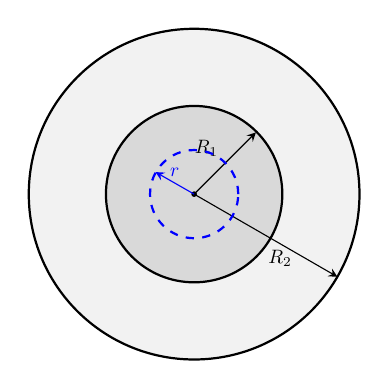
\begin{tikzpicture}[scale=1.4]
            \draw[fill=gray!10, thick] (0,0) circle (1.5);
            \draw[fill=gray!30, thick] (0,0) circle (0.8);
            \draw[fill=black] (0,0) circle (0.02);

            \draw[-stealth] (0,0) -- (0.56, 0.56) node[midway, above left, scale=0.7] {$R_1$};
            \draw[-stealth] (0,0) -- (1.3, -0.75) node[pos=0.6, below, scale=0.7] {$R_2$};

            % Superficie Gaussiana r < R1
            \draw[dashed, blue, thick] (0,0) circle (0.4);
            \draw[-stealth, blue] (0,0) -- (-0.35, 0.2) node[midway, above, scale=0.7] {$r$};
        \end{tikzpicture}
    \end{figure}

    Luego, mediante la Ley de Gauss, se tiene:

    \begin{equation}
        \oiint_S \vec{D} \cdot d\vec{S} = Q_{f, enc}
    \end{equation}

    donde $S$ corresponde a la superficie de la esfera escogida.

    Luego, considerando medio lineal, se tiene que $\vec{D} = \epsilon_1\vec{E}$ (la permitividad usada corresponde a la del material donde se está buscando obtener el campo eléctrico).

    \begin{equation}
        \oiint_S \epsilon_1\vec{E} \cdot d\vec{S} = Q_{f, enc}
    \end{equation}

    Además para simplificar la expresión:

    \begin{enumerate}
        \item El vector del campo eléctrico $\vec{E}$ es paralelo al vector normal de $S$ ($d\vec{S}$) en todo momento, por lo que: $\vec{E} \cdot d\vec{S} = EdS$.

              \begin{equation}
                  \epsilon_1\oiint_S EdS = Q_{f, enc}
              \end{equation}

        \item La magnitud del E es constante en todo punto de la superficie de $S$ debido a que cada punto es equidistante de todas las cargas presentes.

              Por lo que:

              \begin{equation}
                  \epsilon_1E \iint_S dS = Q_{f, enc}
              \end{equation}
    \end{enumerate}

    Luego la integral $\iint_S dS$ corresponde únicamente a el área de la superficie de la esfera $S$, la cual coresponde a $4\pi r^2$.

    Nos queda calcular la magnitud de la carga contenida por la esfera $S$, esta se puede obtener mediante el producto de la densidad de carga volumétrica $\rho_1$ por el volumen encerrado que sigue esta densidad de carga.

    El volumen encerrado corresponde a $\frac{4}{3}\pi r^3$, así, finalmente.

    \begin{align}
        \epsilon_1E \iint_S dS = Q_{f, enc}
        \\
        \epsilon_1E\, 4\pi r^2 = \rho_1\frac{4}{3}\pi r^3
        \\
        E = \frac{\rho_1}{3\epsilon_1}r
    \end{align}

    Finalmente, como el campo es generado por una esfera simétrica, poseerá dirección radial.

    \begin{equation}
        \vec{E} = \frac{\rho_1}{3\epsilon_1}r \;\hat{r}, \qquad \text{con } 0<r<R_1
    \end{equation}

    {\bfseries \large Caso 2: $R_1<r<R_2$.}

    Nuevamente, se debe escoger una superficie donde aplicar la Ley de Gauss, la cual seguirá siendo una esfera de radio $r$, esta será la superficie $C$ (con $R_1<r<R_2$).

    \begin{figure}[H]
        \centering
        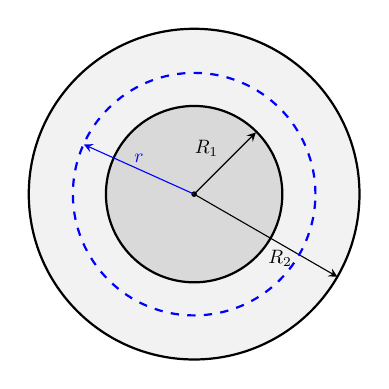
\begin{tikzpicture}[scale=1.4]
            \draw[fill=gray!10, thick] (0,0) circle (1.5);
            \draw[fill=gray!30, thick] (0,0) circle (0.8);
            \draw[fill=black] (0,0) circle (0.02);

            \draw[-stealth] (0,0) -- (0.56, 0.56) node[midway, above left, scale=0.7] {$R_1$};
            \draw[-stealth] (0,0) -- (1.3, -0.75) node[pos=0.6, below, scale=0.7] {$R_2$};

            % Superficie Gaussiana R1 < r < R2
            \draw[dashed, blue, thick] (0,0) circle (1.1);
            \draw[-stealth, blue] (0,0) -- (-1, 0.45) node[midway, above, scale=0.7] {$r$};
        \end{tikzpicture}
    \end{figure}

    Este caso se cumplen las mismas condiciones de simetria en dirección y magnitud del campo en todo punto de la superficie, por lo que por Ley de Gauss se tiene.

    \begin{equation}
        \oiint_C \vec{D} \cdot d\vec{S} = Q_{f, enc} \implies \epsilon_2E \iint_C dS = Q_{f, enc} \label{guia3:p1:eq2}
    \end{equation}

    La integral $\iint_C dS$ nuevamente corresponde a el área de la superficie de la esfera elegida, $4\pi r^2$.

    Sin embargo, la carga encerrada esta vez difiere, pues el núcleo posee una carga dada por la densidad de carga $\rho_1$, mientras que la carga del volumen externo al núcleo está dada por la densidad de carga $\rho_2$.

    Así, la carga total encerrada está dada por la suma de toda la carga correspondiente al núcleo, sumado a la carga del volumen externo al núcleo encerrado por la esfera escogida.

    \begin{itemize}
        \item \textbf{Carga total del núcleo:} Como la superficie encierra totalmente el núcleo de la esfera (de radio $R_1$), el volumen de este será $V_n = \frac{4}{3}\pi R_1^3$.
        \item \textbf{Carga del volumen parcial externo al núcleo:} Aquí estamos encerrando una porcion del volumen cargado externo al núcleo que se extiende desde $R_1$, hasta $r$, el volumen total, lo podemos expresar como la resta entre el volumen de la esfera de radio $r$ y la esfera que no se considera (de radio $R_1$).
              Quedando en $V_{ex, enc} = \frac{4}{3}\pi (r^3 - R_1)$.
    \end{itemize}

    Finalmente, la carga encerrada queda en:
    \begin{gather}
        Q_{f, enc} = \rho_1 V_n + \rho_2 V_{ex, enc}
        \\
        Q_{f, enc} = \rho_1 \frac{4}{3}\pi R_1^3 + \rho_2 \frac{4}{3}\pi (r^3 - R_1)
        \\
        Q_{f, enc} = \frac{4}{3}\pi \left(\rho_1  R_1^3 + \rho_2 (r^3 - R_1)\right)
    \end{gather}

    Volviendo a la expresión de la eq. \ref{guia3:p1:eq2} y reemplazando $Q_{f, enc}$ y el valor de la superficie de la esfera.

    \begin{gather}
        \epsilon_2E \iint_C dS = Q_{f, enc}
        \\
        \epsilon_1E \cdot 4\pi r^2 = \frac{4}{3}\pi \left(\rho_1  R_1^3 + \rho_2 (r^3 - R_1)\right)
        \\
        E = \left(\rho_1  R_1^3 + \rho_2 (r^3 - R_1)\right)\frac{1}{3\epsilon_2 r^2}
        \\
        \vec{E} = \left(\rho_1  R_1^3 + \rho_2 (r^3 - R_1)\right)\frac{1}{3\epsilon_2 r^2} \, \hat{r},\qquad \text{con }R_1<r<R_2
    \end{gather}

    {\bfseries \large Caso 3: $R_2<r$.}

    Por última vez, se debe escoger una superficie donde aplicar la Ley de Gauss, la cual seguirá siendo una esfera de radio $r$, esta será la superficie $F$ (con $R_2<r$).

    \begin{figure}[H]
        \centering
        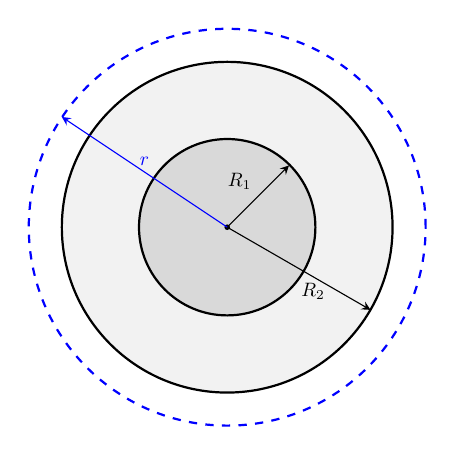
\begin{tikzpicture}[scale=1.4]
            \draw[fill=gray!10, thick] (0,0) circle (1.5);
            \draw[fill=gray!30, thick] (0,0) circle (0.8);
            \draw[fill=black] (0,0) circle (0.02);

            \draw[-stealth] (0,0) -- (0.56, 0.56) node[midway, above left, scale=0.7] {$R_1$};
            \draw[-stealth] (0,0) -- (1.3, -0.75) node[pos=0.6, below, scale=0.7] {$R_2$};

            % Superficie Gaussiana r > R2
            \draw[dashed, blue, thick] (0,0) circle (1.8);
            \draw[-stealth, blue] (0,0) -- (-1.5, 1.0) node[midway, above, scale=0.7] {$r$};
        \end{tikzpicture}
    \end{figure}

    En este caso nuevamente se cumplen las mismas condiciones de simetría de los casos pasado, por lo que por Ley de Gauss se tiene

    \begin{equation}
        \oiint_F \vec{D} \cdot d\vec{S} = Q_{f, enc} \implies \epsilon_0E \iint_F dS = Q_{f, enc} \label{guia3:p1:eq3}
    \end{equation}

    La integral $\iint_F dS$ corresponde al área de la superficie de la esfera elegida, $4\pi r^2$.

    Finalmente la carga encerrada corresponde a toda la carga en el volumen de la esfera (nucleo mas volumen exterior), por lo que únicamente es necesario obtener el volumen total de la parte exterior al núcleo.

    Sabemos que el volumen del núcleo es $V_n = \frac{4}{3}\pi R_1^3$. Luego el volumen total de la parte de la esfera exterior al núcleo correponderá a $V_{ex} = \frac{4}{3}\pi (R_2^3 - R_1^3)$.

    Por lo tanto:

    \begin{gather}
        Q_{f, enc} = \rho_1 V_n + \rho_2 V_{ex}
        \\
        Q_{f, enc} = \rho_1 \frac{4}{3}\pi R_1^3 + \rho_2 \frac{4}{3}\pi (R_2^3 - R_1^3)
    \end{gather}

    Volviendo a la expresión de la Ley de Gauss eq. \ref{guia3:p1:eq3}.

    \begin{gather}
        \epsilon_0E \iint_F dS = Q_{f, enc}
        \\
        \epsilon_0E \iint_F dS = Q_{f, enc}
        \\
        \epsilon_0 E \cdot 4\pi r^2 = \left(\rho_1 \frac{4}{3}\pi R_1^3 + \rho_2 \frac{4}{3}\pi (R_2^3 - R_1^3)\right)
        \\
        \epsilon_0 E \cdot 4\pi r^2 = \frac{4}{3}\pi \left(\rho_1 R_1^3 + \rho_2 (R_2^3 - R_1^3)\right)
        \\
        E = \left(\rho_1 R_1^3 + \rho_2 (R_2^3 - R_1^3)\right)\frac{1}{3\epsilon_0r^2}
        \\
        \vec{E} = \left(\rho_1 R_1^3 + \rho_2 (R_2^3 - R_1^3)\right)\frac{1}{3\epsilon_0r^2}\;\hat{r},\qquad \text{con }R_2<r
    \end{gather}
\end{solucion}

\begin{problema}[Campo Eléctrico debido a una Línea Infinita]
    Considere un cable recto, muy delgado e infinitamente largo, que posee una densidad lineal de carga $\lambda$ (uniforme en toda su longitud).

    Obtenga una expresión para la magnitud de campo eléctrico a una distancia $r$ del cable.

    \begin{figure}[H]
        \centering
        \shorthandoff{>}
        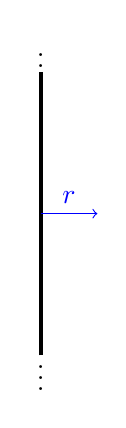
\begin{tikzpicture}[scale=0.6]
            % Línea infinita de carga (el cable) con puntos suspensivos
            \draw[ultra thick] (0, -3) -- (0, 3);
            \node at (0, 3.3) {$\vdots$};
            \node at (0, -3.3) {$\vdots$};

            % Etiqueta del radio gaussiano r
            \draw[->, blue] (0,0) -- (1.2, 0) node[midway, above] {$r$};
        \end{tikzpicture}
        \shorthandon{>}
    \end{figure}
\end{problema}

\begin{solucion}
    Como es habitual con el uso de la Ley de Gauss, es necesario escoger una superficie donde aplicar el análisis, para problemas con líneas infinitas, la superficie adecuada corresponde a un cilindro del mismo radio dado en el enunciado $r$ y largo \textbf{} $L$.

    \begin{figure}[H]
        \centering
        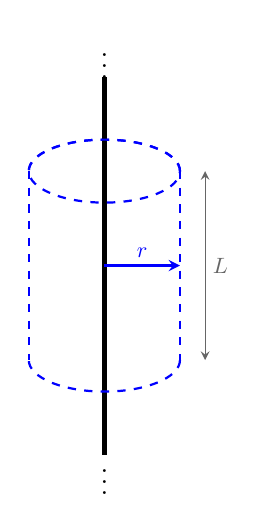
\begin{tikzpicture}[scale=0.8]
            % Superficie Gaussiana: Cilindro (parte trasera)
            \draw[blue, thick, dashed] (1.2, 1.5) arc (0:180:1.2 and 0.5);

            % Línea infinita de carga
            \draw[ultra thick] (0, -3) -- (0, 3);
            \node at (0, 3.3) {$\vdots$};
            \node at (0, -3.3) {$\vdots$};

            % Superficie Gaussiana: Cilindro (cuerpo y parte frontal)
            \draw[blue, thick, dashed] (-1.2, 1.5) -- (-1.2, -1.5);
            \draw[blue, thick, dashed] (1.2, 1.5) -- (1.2, -1.5);
            \draw[blue, thick, dashed] (0, 1.5) ellipse (1.2 and 0.5);
            \draw[blue, thick, dashed] (1.2, -1.5) arc (0:-180:1.2 and 0.5);

            % Etiqueta del radio r
            \draw[-stealth, blue, thick] (0,0) -- (1.2, 0) node[midway, above, scale=0.8] {$r$};

            % Etiqueta del largo L
            \draw[stealth-stealth, black!60] (1.6, 1.5) -- (1.6, -1.5) node[midway, right, scale=0.8] {$L$};
        \end{tikzpicture}
    \end{figure}

    Luego, siguiendo con la Ley de Gauss se tiene
    \begin{equation}
        \oiint_S \vec{D} \cdot d\vec{S} = Q_{f, enc}
    \end{equation}
    donde $S$ corresponde a la superficie del cilindro escogido.

    Inicialmente notamos que la superficie del cilindro consta de 3 partes, la tapa inferior, superior y el manto, cada una de estas tapas posee vector normal a su superficie distinto entre si, pero identificado, por lo cual podemos separar la integral de superficie entre sus componentes.
    \begin{equation}
        \iint_{T. inf} \vec{D} \cdot d\vec{S} + \iint_{T. sup} \vec{D} \cdot d\vec{S} + \iint_{Mant} \vec{D} \cdot d\vec{S} = Q_{f, enc}
    \end{equation}

    Sabemos que en el vacío $\vec{D}=\epsilon_0\vec{E}$.

    Luego, analizando que ocurre en cada superficie notamos lo siguiente:

    \begin{itemize}
        \item \textbf{Dirección del Campo Eléctrico:} Lo primero que podemos notar es que la dirección del campo eléctrico sólo puede contener dirección radial y \textbf{horizontal} (mas o menos la misma dirección que la flecha azul en la figura) a lo largo de todo el eje vertical.
        \item \textbf{Dirección del vector normal a la superficie de ambas tapas:} Visualmente podemos notar que el vector normal a la superficie en todo punto de tanto la tapa superior como inferior corresponde a un vector que únicamente contiene componente \textbf{vertical}.
        \item \textbf{Conclusión:} Como en todo momento el vector de campo eléctrico posee dirección horizontal y radial, mientras que los vectores normales a las superficies de las tapas son verticales, el producto escalar entre $\vec{E}$ y $d\vec{S}$ siempre será nulo: $\vec{E}\cdot d\vec{S}$. Por lo tanto
              \begin{equation}
                  \iint_{T.inf}\epsilon_0\vec{E}\cdot d\vec{S} = \iint_{T.sup}\epsilon_0EdS = 0
              \end{equation}
    \end{itemize}

    Quedando
    \begin{equation}
        \iint_{Mant} \epsilon_0 \vec{E} \cdot d\vec{S} = Q_{f, enc} \label{guia3:p2:eq1}
    \end{equation}

    Luego queda analizar la integral de superficie sobre el manto.

    \begin{itemize}
        \item \textbf{Dirección del vector normal a la superficie del manto:} El vector normal de la superficie del manto se puede notar que es completamente \textbf{radial} y \textbf{horizontal}, por lo que al igual que el campo eléctrico, estos son completamente paralelos, por lo tanto $\iint_{Mant} \epsilon_0\vec{E}\cdot d\vec{S} = \iint_{Mant} \epsilon_0EdS$.
        \item \textbf{Magnitud del campo eléctrico en cada punto de la superficie:} Otra cosa que es necesario notar es que la magnitud del campo eléctrico en \textbf{todo} punto de la superficie es completamente constante, por lo cual es independiente de la integral, por lo tanto $\epsilon_0E \iint_{Mant}dS$. Así finalmente $\iint_{Mant}dS$ corresponde únicamente a la superficie del manto del cilindro, dada por $2\pi rL$.
    \end{itemize}

    Volviendo a la ecuación \ref{guia3:p2:eq1} se tiene

    \begin{gather}
        \iint_{Mant} \epsilon_0 \vec{E} \cdot d\vec{S} = Q_{f, enc}
        \\
        \epsilon_0E \iint_{Mant}dS = Q_{f, enc}
        \\
        \epsilon_0E 2\pi rL = Q_{f, enc}
    \end{gather}

    Finalmente, la cantidad de carga encerrada corresponde únicamente a la sección de largo $L$ interna a la superficie cilíndrica, mediante la densidad de carga lineal llegamos a que la carga encerrada es $\lambda L$.

    Por lo tanto, la expresión final queda
    \begin{gather}
        \epsilon_0E 2\pi rL = Q_{f, enc} \implies \epsilon_0E 2\pi rL = \lambda L \implies E = \frac{\lambda}{2\pi\epsilon_0 r}
    \end{gather}

    Como el campo apunta de forma radial y horizontal, en \textit{coordenadas cilíndricas} se expresa
    \begin{equation}
        \vec{E} = \frac{\lambda}{2\pi\epsilon_0 r} \;\hat{r}
    \end{equation}
\end{solucion}

\begin{problema}[Campo Eléctrico debido a un Plano Infinito]
    Se tiene una placa plana infinita de material aislante, la cual posee una densidad superficial de carga $\sigma$ uniforme.

    Encuentre la magnitud del campo eléctrico $E$ a una distancia $z$ de la placa.

    \begin{figure}[H]
        \centering
        \shorthandoff{>}
        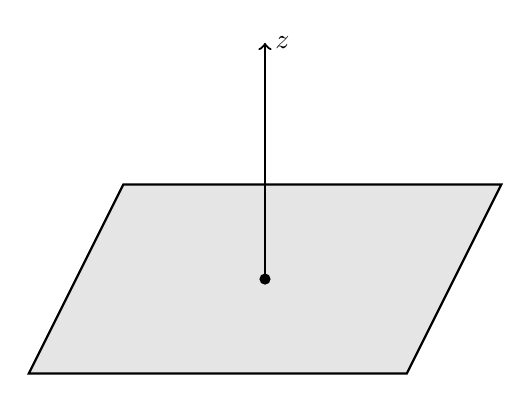
\begin{tikzpicture}[scale=1.2]
            % Plano infinito en z=0 (acostado en perspectiva)
            \draw[fill=gray!20, thick] (-2.5, -1) -- (1.5, -1) -- (2.5, 1) -- (-1.5, 1) -- cycle;

            % Parte saliendo hacia arriba
            \draw[->, thick] (0, 0) -- (0, 2.5) node[right] {$z$};

            % Punto de origen en el plano
            \filldraw[black] (0,0) circle (1.5pt);
        \end{tikzpicture}
        \shorthandon{>}
    \end{figure}
\end{problema}

\begin{solucion}
    Como corresponde con el uso de la Ley de Gauss, es necesario escoger una superficie donde aplicar el análisis, para problemas con planos infinitos, la superficie adecuada corresponde a un cilindro de radio arbitrario $r$ y largo arbitrario $L$.

    \textit{Nota: La selección de superficie está completamente asociada al sistema de coordenadas predominante en cada análisis, por lo que para el plano infinito corresponde a un cubo de largo $L$, sin embargo el uso del cilindro tiene exactamente los mismos resultados con un desarrollo más breve.}

    \begin{figure}[H]
        \centering
        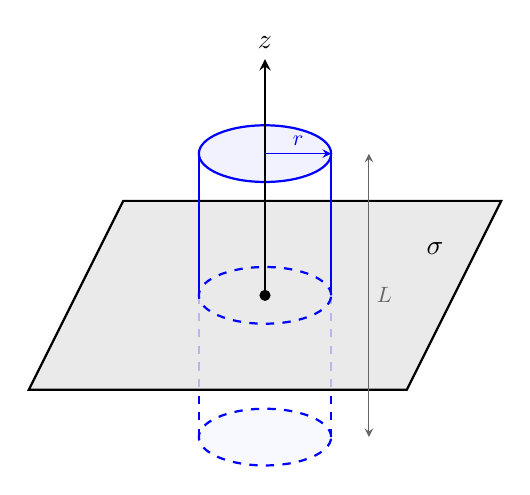
\begin{tikzpicture}[scale=1.2]
            % 1. Parte inferior del cilindro (detrás del plano)
            \draw[blue, thick, dashed, fill=blue!5, fill opacity=0.5] (0,-1.5) ellipse (0.7 and 0.3);
            \draw[blue, thick, dashed] (-0.7,-1.5) -- (-0.7,0);
            \draw[blue, thick, dashed] (0.7,-1.5) -- (0.7,0);

            % 2. El Plano Infinito (se dibuja "en medio")
            \draw[fill=gray!20, thick, fill opacity=0.8] (-2.5, -1) -- (1.5, -1) -- (2.5, 1) -- (-1.5, 1) -- cycle;

            % Intersección (elipse donde el cilindro toca el plano)
            \draw[blue, thick, dashed] (0,0) ellipse (0.7 and 0.3);

            % 3. Parte superior del cilindro (al frente del plano)
            \draw[blue, thick] (-0.7,0) -- (-0.7,1.5);
            \draw[blue, thick] (0.7,0) -- (0.7,1.5);
            \draw[blue, thick, fill=blue!10, fill opacity=0.5] (0,1.5) ellipse (0.7 and 0.3);

            % 4. Ejes y etiquetas
            % Eje z
            \draw[-stealth, thick] (0, 0) -- (0, 2.5) node[above] {$z$};
            \filldraw[black] (0,0) circle (1.5pt);

            % Cota de Radio r
            \draw[-stealth, blue] (0, 1.5) -- (0.7, 1.5) node[midway, above, scale=0.8] {$r$};

            % Cota de Largo L
            \draw[stealth-stealth, black!60] (1.1, 1.5) -- (1.1, -1.5) node[midway, right, scale=0.8] {$L$};

            % Indicador de densidad sigma
            \node at (1.8, 0.5) {$\sigma$};
        \end{tikzpicture}
    \end{figure}

    Por la Ley de Gauss tenemos:

    \begin{equation}
        \oiint_S \vec{D}\cdot d\vec{S} = Q_{f, enc}
    \end{equation}

    Inicialmente notamos que la superficie del cilindro consta de 3 partes, la tapa inferior, superior y el manto, cada una de estas tapas posee vector normal a su superficie distinto entre si, pero identificado, por lo cual podemos separar la integral de superficie entre sus componentes.

    \begin{equation}
        \iint_{T. inf} \vec{D} \cdot d\vec{S} + \iint_{T. sup} \vec{D} \cdot d\vec{S} + \iint_{Mant} \vec{D} \cdot d\vec{S} = Q_{f, enc}
    \end{equation}

    Sabemos que en el vacío $\vec{D}=\epsilon_0\vec{E}$.

    Luego, analizando que ocurre en cada superficie notamos lo siguiente:

    \begin{itemize}
        \item \textbf{Dirección del Campo Eléctrico:} Lo primero que podemos notar es que la dirección del campo eléctrico sólo puede tener dirección \textbf{vertical}, ya que toda carga responsable de producir componente horizontal en el espacio tendrá una carga por otro lado que anule esta misma.
        \item \textbf{Dirección del vector normal a la superficie de ambas tapas:} Visualmente podemos notar que el vector normal a la superficie en todo punto de tanto la tapa superior como inferior corresponde a un vector que únicamente contiene componente \textbf{vertical}.
        \item \textbf{Conclusión:} Como en todo momento el vector de campo eléctrico posee dirección paralela al vector normal (y mismo sentido) a la superficie de las tapas, el producto escalar queda como $\vec{E}\cdot d\vec{S} = EdS$ y además, el resultado de las integrales es el mismo. Por lo tanto
              \begin{equation}
                  \iint_{T.inf}\epsilon_0\vec{E}\cdot d\vec{S} = \iint_{T.sup}\epsilon_0\vec{E}\cdot d\vec{S} = \iint_{T}\epsilon_0EdS
              \end{equation}
        \item \textbf{Magnitud del campo eléctrico en cada punto de la superficie:} También es posible observar que, si el cilindro escogido atraviesa el plano justo en medio de este, la magnitud del campo eléctrico en \textbf{todo} punto de la superficie de las tapas es constante, por lo cual es independiente de las integrales, por lo tanto $\epsilon_0E \iint_{T}dS$. Y, finalmente $\iint_{T}dS$ corresponde únicamente a la superficie de la tapa del cilindro, dada por $\pi r^2$.
    \end{itemize}

    De todo esto, nos queda:

    \begin{gather}
        \iint_{T. inf} \vec{D} \cdot d\vec{S} + \iint_{T. sup} \vec{D} \cdot d\vec{S} + \iint_{Mant} \vec{D} \cdot d\vec{S} = Q_{f, enc}
        \\
        \iint_{T} \epsilon_0EdS + \iint_{T} \epsilon_0EdS + \iint_{Mant} \epsilon_0\vec{E} \cdot d\vec{S} = Q_{f, enc}
        \\
        2 \epsilon_0E\iint_{T}dS + \iint_{Mant} \epsilon_0\vec{E} \cdot d\vec{S} = Q_{f, enc}
        \\
        2\epsilon_0E\pi r^2 + \iint_{Mant} \epsilon_0\vec{E} \cdot d\vec{S} = Q_{f, enc}
    \end{gather}

    Posteriormente con la integral relacionada a manto del cilindro elegido y la carga encerrada se tiene:

    \begin{itemize}

        \item \textbf{Dirección del vector normal a la superficie del manto:} El vector normal de la superficie del manto se puede notar que es completamente \textbf{radial} y \textbf{horizontal}, y como el vector del campo eléctrico en todo punto es vertical, el producto punto siempre dará un resultado \textbf{nulo}, por lo tanto $\iint_{Mant} \epsilon_0\vec{E}\cdot d\vec{S} = 0$.

        \item \textbf{Carga Encerrada:} La carga encerrada corresponde al toda la contenida por la circunferencia formada por el cruce entre el cilíndro y el plano, circunferencia del mismo radio del cilindro ($r$). Asi, junto con la densidad de carga superficial $\sigma$, la carga contenida es: $Q_{f, enc} = \sigma \pi r^2$.
    \end{itemize}

    Juntando todo esto, tenemos

    \begin{gather}
        2\epsilon_0E\pi r^2 + \iint_{Mant} \epsilon_0\vec{E} \cdot d\vec{S} = Q_{f, enc}
        \\
        2\epsilon_0E\pi r^2 = \sigma \pi r^2
        \\
        E = \frac{\sigma}{2\epsilon_0}
    \end{gather}

    Como el campo tiene solo componente vertical, finalmente:
    \begin{equation}
        \vec{E} = \frac{\sigma}{2\epsilon_0} \,\hat{z}
    \end{equation}

    \textit{Curiosidad: El campo eléctrico debido a un plano infinito \textbf{no depende} de la distancia a la que se esté del plano, esto es una utilidad que será considerada en los contenidos de condensadores/capacitores.}
\end{solucion}

\end{document}